% !TEX root = main.tex

\section{基础概念}
\subsection{训练集与测试集}
\begin{itemize}
	\item 留出法(hold-out):直接将数据集划分为两个互斥的集合,一个作为训练集,另一个作为测试集
	\begin{itemize}
		\item 注意数据分布的一致性,通过多次随机划分取平均保证
		\item 通常用$2/3\thicksim 4/5$的样本用于训练,其余用作测试
	\end{itemize}
	\item 交叉验证法(cross validation)/$k$折(fold)交叉验证:划分为$k$个互斥子集,其中$k-1$个用于训练,最后一个用于验证,训练$k$次,对这$k$次结果取平均
	\begin{itemize}
		\item 通常采用10次10折交叉验证,每次都换划分方式,确保随机性
	\end{itemize}
	\item 自助法(bootstrapping):从原始数据集中放回采样得到新数据集作为测试集
	\begin{itemize}
		\item 在数据集较小的、难以有效划分训练/测试集时比较有用
		\item 但改变了初始数据集分布,会引入估计偏差
	\end{itemize}
\end{itemize}

注意:通常将习得模型实际使用中遇到的数据称为测试集,而将训练的数据划分为训练集与验证集(validation)

\subsection{参数选择}
参数通常包括
\begin{itemize}
	\item 模型本身的参数(parameter):通过学习改变
	\item 超参数(superparameter):预先设定,调参实际上就是在选择算法
\end{itemize}

\subsection{性能度量}
\begin{itemize}
\item 回归:通常采用均方误差(MSE)
\item 分类:错误率、精度
\end{itemize}

对于二分类问题,有混淆矩阵(confusion matrix)
\begin{center}
\begin{tabular}{|c|c|c|}\hline
& 预测正 & 预测反\\\hline
真实正 & TP(真正例) & FN(假反例)\\\hline
真实反 & FP(假正例) & TN(真反例)\\\hline
\end{tabular}
\end{center}
\[\begin{aligned}
\text{查准率}P&=\frac{TP}{TP+FP}\\
\text{查全率}R&=\frac{TP}{TP+FN}
\end{aligned}\]

为了衡量机器学习算法的泛化性能,需要知道以下指标:
\begin{itemize}
	\item 方差(variance):度量同样大小的训练集的变动所导致的学习性能的变化,即刻画数据扰动所造成的影响
	\[\Var{\vx}=\mathbb{E}_D\lrs{\lrp{f(\vx;D)-\bar{f}(\vx)}^2}\]
	\item 偏差(bias):度量学习算法的期望预测和真实结果的偏离程度,即刻画学习算法本身的拟合能力
	\[b^2(\vx)=\lrp{\bar{f}(\vx)-y}^2\]
	\item 噪声(noise):表达在当前任务上任何学习算法所能达到的期望泛化误差的下界
	\[\eps^2=\mathbb{E}_D\lrs{\lrp{y_D-y}^2}\]
\end{itemize}

泛化误差可以分解为
\[E(f;D)=b^2(\vx)+\Var{\vx}+\eps^2\]
即泛化性能是由学习算法的能力、数据的充分性及学习任务本身的难度决定的
\begin{figure}[H]
\centering
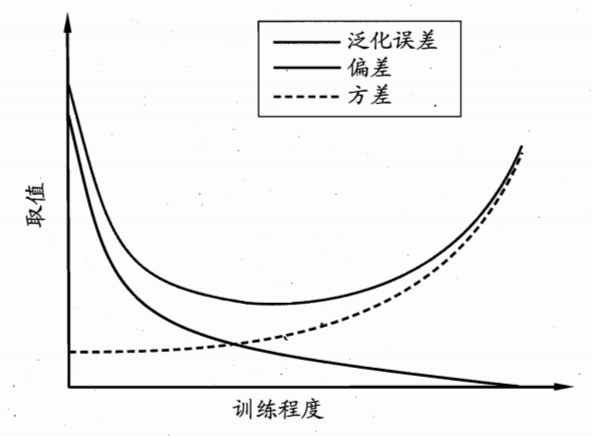
\includegraphics[width=0.4\linewidth]{fig/bias-var.png}
\end{figure}